\chapter{Symbolic knowledge representation}
\label{chapt|krs}

\fxnote{Support material: \emph{What is a knowledge representation} by Davis,
Shrobe and Szolovits,
\url{http://groups.csail.mit.edu/medg/ftp/psz/k-rep.html}}

\section{What do we call "knowledge"?}
\label{sect|on-knowledge}

\subsection{The Concept of Knowledge}
\label{sect|knowledge}


Since we will discuss at length the concept of knowledge in the context
of robotics in the coming pages, it is useful to make our terminology explicit.  No general
agreement on a definition of ``knowledge'' exists. In our context, we call
``knowledge'' \emph{an explicit set of interrelated logical facts that are
meaningful to the robot executive controller} (by \emph{meaningful} we mean
that can possibly be interpreted to lead to a purposeful action).

The relation of \emph{data} and \emph{information} to knowledge is a debated
epistemology question (the interested reader is invited to refer to the
Wikipedia page on the ``DIKW'' hierarchy). In this thesis, we will associate
data to low-level material like raw sensor output, and information to
uncontextualized symbolic facts.

To give a example, image a human watching at a book and being tracked by a
Kinect sensor: the pose of the human skeleton in the world would be the data,
the fact \concept{looksAt(human, book)} as computed by a geometric reasoning
module would be the information, the fact \concept{looksAt(john,
war\_and\_peace)}, fully grounded and connected to the whole knowledge base of
the robot would be proper knowledge.

Note that the origins of AI where in purely symbolic models, that were
not usable either. Rich interleaving between geometric reasoning and symbolic
models is required.

...

While \emph{knowledge} has no general definition that researchers agree on, for
our own purposes we define knowledge as \emph{information interpreted in the
cultural and social context of the robot}, where information is a
\emph{statement} or an \emph{assertion} about the world\footnote{In this paper,
statements are always triples \stmt{subject predicate object}, \ie binary
relations between entities.}. In practical terms, knowledge is made of
statements that are \emph{contextualized}, if possible \emph{synthesized}, and
\emph{limited} to a domain of validity. These three features have important 
consequences for the way a knowledge representation and storage system must 
be designed. Let us examine them:

\paragraph{Contextualizing} is the ability for a cognitive system to connect a
fact with a \emph{cultural context}, an \emph{interpretive scope} and the set
of other facts previously acquired by the agent.

Since machines are limited to syntactic (in contrast to semantic)
processing, we are mostly looking for a syntactic (\ie, based on symbols)
matching between concepts representations (in our case, sets of alphanumeric
characters).\fxfatal{il faut sans doute évoquer ici la relation
sémantique/syntactique que propose Choamsky}.

We call \textit{cultural context} a broad set of common, general facts that are
considered widely accepted among the interactors (\eg ``bottles may contain
water''). This knowledge is often referred as \emph{common-sense knowledge}.

By \emph{interpretive scope} we mean that a concept may have different
interpretations depending on the agent, the current situation or the time frame
the statement belongs to. Since a fact in one scope can be different (or even
inconsistent) with a fact in another scope (for instance, one object can be
visible for the robot and invisible for another agent), the underlying
knowledge representation system must properly handle these interpretive
frameworks.

Note that the focus of ORO is on enabling such context to be
effectively represented rather than actually identifying the current context.
While several approaches for building contextualized knowledge are proposed in this
paper (symbolic environment interpretation, perspective taking, grounded
natural language resolution, self-awareness of its own activity), much remains
to be done for a robot to actually identify its current context as well as
contexts that may be referred to.

\paragraph{Synthesis} corresponds to the identification of facts and their
components (concepts and predicates) with respect to other facts. For instance,
if the robot observes a human sitting down at a table, and at the same time, we
tell it that ``Peter is sitting at the table'', we would like the robot to
infer that ``Peter'' may be the name of the human. \textit{Synthesis}
refers to the fact that several, \textit{a priori} uncorrelated, facts
must be associated with the same common concept. This process requires the
ability to control the logical consistency of the knowledge corpus. To
continue with the previous example,  if we add the fact that the human that
is sitting is a woman, the synthesis ``Peter is the name of the human'' is
not valid anymore.

\paragraph{Domain of validity} specifies the scope in which
 information is (believed to be) true. It covers several aspects: temporal,
situational and probabilistic. While related to the previous concept of
\emph{interpretive scopes}, the domain of validity addresses the question
whether a fact must be or not considered in a given context. This validity
limitation is not usually carried by the fact itself. In the previous example,
for instance, the robot observes a human sitting at a table.  The fact ``a
human is sitting at the table'' is true only for a limited period of time,
until the human stands up. This period of time is not directly accessible
(the robot does not know how long the human plans to stay), but the
knowledge representation must be able to deal with this uncertainty and
should explicitly label this fact as being limited in time.

To know if a fact is permanent or transitional (as defined by Pollock
\cite{Pollock1998}, page 51) is difficult (especially
considering that a feature may be considered as permanent or not depending of
the context: within the situation ``a familly meal''\fxfatal{Check
translation!}, the fact ``the human is sitting at the table'' could be
considered as permanent. Conversely, ``ground is static'' is generally
considered as a permanent fact, expect if we are talking of planetary mechanics
for instance. The difficulty lies in the selection of the relevant situation
in which reasoning must be carried out at a given time) and have currently to
be defined in the cultural background of the robot.

These three aspects lead us to envisage a knowledge representation system
characterized by the following abilities: 
\begin{itemize}
	\item represent raw information,
	\item render a general cultural background, in the form of common-sense knowledge,
	\item attach interpretive scopes to new statements,
	\item add and connect new statements to knowledge already present,
	\item store restrictions on the domain of validity of the knowledge.
\end{itemize}

Besides, the following active processes would be desirable:
\begin{itemize}
	\item acquire and maintain knowledge perceived from the physical world or
	retrieved from other sources (interaction with other agents, web-based contents,...)
	\item synthesize facts as much as possible,
	\item monitor contexts and accordingly manage the validity of the stored knowledge,
	\item ensure the logical consistency of the knowledge repository, and
	explicit inconsistencies when required\footnote{One may argue that the real world is 
	inherently inconsistent. In this article, we make a
	\textit{consistent world} assumption, in order to leverage reasoning
	capabilities of the first-order logics. This is supported by the natural
	tendency of humans themselves to provide a consistent explanation of their
	world.}.
\end{itemize}

This list does not cover all the possible features that could be exposed by a
symbolic knowledge management system. Bio-inspired memory management (the
ability to forget or reinforce knowledge) or curiosity (the ability to identify
lacking knowledge and actively trigger behaviours to acquire it --Hawes et
al.~\cite{Hawes2011} have contributed in this area with \emph{Dora}, a
robot endowed with motivation mechanisms to explore unknown regions of
the environment--), to give some examples, could arguably be added to the list.
However, this first analysis sets a convenient reference frame to understand
and evaluate knowledge representation systems, including the \textsc{ORO}
knowledge management system we propose.

\subsection{The Semantic Robot}
\label{sect|semantic}


One concept, several symbols: cf multilingual support of ORO server \ref{sect|multilingual}.


%%%%%%%%%%%%%%%%%%%%%%%%%%%%%%%%%%%%%%%%%%%%%%%%%%%%%%%%%%%%%%%%%%%%%%%%%%%%%%%%%%%%%%%%%%%
%%%%%%%%%%%%%%%%%%%%%%%%%%%%%%%%%%%%%%%%%%%%%%%%%%%%%%%%%%%%%%%%%%%%%%%%%%%%%%%%
\section{Towards Analysing the Knowledge Representation Requirements}
\label{sect|krs-related-work}


The idea of \emph{Cognitive Robotics} was coined in the early 1990s by Reiter.
In a chapter on that subject in \emph{Fondations of Artifical
Intelligence}~\cite{Levesque2008}, Levesque reminds about the manifesto they
wrote together in 1998:

\begin{quotation}

    Central to this effort is to develop an understanding of the relationship
    between the knowledge, the perception, and the action of [\ldots] a robot. The
    sorts of questions we want to be able to answer are

    \begin{itemize} 

        \item to execute a program, what information does a robot need to have
        at the outset vs. the information that it can acquire \emph{en route}
        by perceptual means?

        \item what does the robot need to know about its environment vs. what
        need only be known by the designer?

        \item when should a robot use perception to find out if something is
        true as opposed to reasoning about what it knows was true in the past?

        \item when should the inner workings of an action be available to the
        robot for reasoning and when should the action be considered primitive
        or atomic?

    \end{itemize}

    and so on. With respect to robotics, our goal (like that of many in AI) is
    \emph{high-level robotic control}: develop a system that is capable of
    generating actions in the world that are appropriate as a function of some
    current set of beliefs and desires.

\end{quotation}

To be answered, those questions have in common one prerequisite: the robot must
be able to manipulate \emph{explicitly} knowledge, and hence, need a way to
represent the knowledge.

This section focuses on this knowledge representation issue: we aims at first
establishing a comprehensive typology of representational needs for
robotics in the specific context of service robotics, and then at painting the
current landscape of approaches to the knowledge representation problem in the
research community.

While not strictly focused on knowledge in the context of
service robotics, several previous work have sketched lists of important items for cognitive robots.

Heintz et al.~\cite{Heintz2008} define
\emph{knowledge processing middlewares} as systems supporting ``declarative
specifications for flexible configuration and dynamic reconfiguration of
context dependent processing at many different levels of abstraction''. They
identify six characteristics: the system must be able to merge informations
from different, possibly distributed sources; it should support quantitative as
well as qualitative processing of information, it should offer bottom-up and
top-down processing, it should be able to deal with uncertainty, allow for
``flexible configuration and reconfiguration'' (which require what we call
\emph{non-monotonicity} in this article) and finally meta-knowledge and
introspective capacities (``declarative specification of the processing
functionalities''). In this paper, we focus our analysis on similar system with
however an emphasize on the symbolic capabilities.

Several surveys compare global cognitive architectures (\cite{Vernon2007, Chong2009}).
Vernon et al.~\cite{Vernon2007} split these architectures into two broad
categories: the \emph{cognitivist} ones (where cognition is considered as an
explicit computation problem, often based on symbol manipulation), and the
\emph{emergent} ones (where cognition only exists as a result of the
interaction of the system with its environment). The approaches presented in
this paper are, at a few exceptions, prototypical \emph{cognitivist} approaches
that aim at making knowledge explicit within the robot architecture. Vernon et
al. propose twelve \emph{characteristics of cognitive system} to compare
architectures. Amongst them, they mention the \emph{inter-agent epistemology} (how
the structure of the world is captured in a representation and shared), the
relation to \emph{embodiment}, the ability to \emph{anticipate} and to
\emph{adapt}, and the mechanisms of \emph{motivation}. While presented at the
level of the whole robotic architecture, these features also translate into
knowledge representation strategies and are relevant to our study.
\fxwarning{Detail Chong here}

At an even broader scope, several authors from fields that are connected to robotics
have previously listed desirable features of artificial systems aiming at
rich cognitive abilities.

For instance, in~\cite{McCarthy2007}, McCarthy recently listed the challenges
he identifies on the road to a \emph{human-level AI}.

\begin{itemize}

	\item the ability to \emph{"operate successfully in the common sense
	informatic situation"},

	\item the necessity of relying on mathematical logic, as the most fruitful
	formalism for machine intelligence,

	\item the ability to deal with \emph{approximate concepts and approximate
	theories} (that would include representing them, and reasoning with them),

	\item non-monotonic reasoning,

	\item what McCarthy calls \emph{Elaboration Tolerance}: the ability to
	extend \emph{on demand} the closed domain of interpretation for a
	given assertion,

	\item the ability to formalize and reason about contexts,

	\item reasoning about events, and in particular, actions,

	\item the capacity of introspection,

	\item and finally, he points the issue of giving computer the right
	heuristics for decision making.

\end{itemize}

Coming from the perspective of natural language processing in situated context,
Roy and Reiter, in~\cite{Roy2005}, summarize what they see as the main
challenges to be tackled by KRS: cross-modal representation systems,
association of words with perceptual and action categories (\emph{grounding}),
modeling of context, definition of the right granularity of models, integration
of temporal modeling and planning, ability to match past (learned) experiences
with the current interaction and ability to take into account the human
perspective.

Knowledge representation systems in robotics are concerned by most, if not all,
of these points, and we shall indeed mention them in our typology, in slightly
reformulated ways.


%%%%%%%%%%%%%%%%%%%%%%%%%%%%%%%%%%%%%%%%%%%%%%%%%%%%%%%%%%%%%%%%%%%%%%%%%%%%%%%%%%%%%%%%%%%
%%%%%%%%%%%%%%%%%%%%%%%%%%%%%%%%%%%%%%%%%%%%%%%%%%%%%%%%%%%%%%%%%%%%%%%%%%%%%%%%
\section{A Typology of Knowledge Representation Requirements for Robotics}
\label{sect|features}
We now want to organize requirements from this imaginary cooking scenario where
numerous desirable features for a knowledge representation system for robotics
have been identified without any particular order.

This section proposes a more formal typology of desirable features for a such a
system. For each feature, we provide a short definition along with links to
relevant literature.

Table~\ref{table|contribution-by-systems}, at the end of the article,
summarizes all these features with the main domain of contribution of each
surveyed KRS.

As previously mentioned, we propose six main categories.

\begin{scriptsize}
\begin{center}
\begin{tikzpicture}[taxonomy]
    %[edge from parent fork east]
    %every node/.style={fill=black!30,rounded corners},
    %[parent anchor=east,child anchor=west,grow=east,
    %edge from parent/.style={thick,draw}]
    \node [taxon] {Dimensions}
        child {node [taxon] {{\bf F}. Instantiation}}
        child {node [taxon] {{\bf E}. Integration}}
        child {node [taxon] {{\bf D}. Acquisition}}
        child {node [taxon] {{\bf C}. Reasoning}}
        child {node [taxon] {{\bf B}. Representation}}
        child {node [taxon] {{\bf A}. Expressiveness}};
\end{tikzpicture}
\end{center}
\end{scriptsize}

\subsection{Expressiveness: What Can be Represented?}
\label{sect|expressiveness}

\begin{scriptsize}
\begin{center}
\begin{tikzpicture}[taxonomy]
    \node [taxon] {\bf A. Expressiveness}
            child {node [taxon] {{\bf A.5}. Meta-cognition}}
            child {node [taxon] {{\bf A.4}. Uncertainty}}
            child {node [taxon] {{\bf A.3}. OWA/CWA}}
            child {node [taxon] {{\bf A.2}. Expressive power}}
            child {node [taxon] {{\bf A.1}. Logic formalism}};
\end{tikzpicture}
\end{center}
\end{scriptsize}


\subsubsection{Main Logic Formalisms}

The main role of a knowledge representation system is to provide an adequate
representation system to store facts and concepts that can be informally
described in natural language.

Formal logic aims at providing such a representation system with the added
value of providing a tractable support for inference and reasoning.

Most (but not all) of the systems we survey rely on a particular logic
formalism. The choice of the formalism has a strong impact, on one side, on the
range of ideas that can be expressed conveniently (\emph{practical
expressiveness}) or at all (\emph{theoretical expressiveness}), on the other
side, on the ability to solve the inference problem (called
\emph{satisfiability}: is a given logical sentence true in my model?) in a
tractable manner.

A large number of logic formalism do exist, we shall summarize below the most
relevant ones for systems actually deployed in current robotic architectures.

\emph{Predicate logic} is the family of logic formalisms the most commonly
found in knowledge representation. It distinguishes itself from the simpler
\emph{propositional logic} by the use of quantification to increase generality.
\emph{First-order logic} (FOL) is the subpart of \emph{predicate logic} where the
objects of \emph{predicates} (or \emph{formulae}) are simple \emph{terms},
while in \emph{higher-order logics}, predicates can be themselves objects of
other predicates.

\emph{Horn clauses} are an important subset of FOL because the satisfiability
of a set of such clauses is a $P$-complete problem (\ie practically tractable).
A Horn clause is a disjunction of literals (a \emph{clause}) with at most one
positive literal: $\neg p \lor \neg q \lor \cdots \lor \neg t \lor u$, which
can also be represented as $(p \land q \land \cdots \land t) \rightarrow u$.
Important logic programming languages like Prolog are based on Horn clauses.

The family of \emph{Description Logics}~\cite{Baader2008} also play an
important role. It is also a subset of the first-order logic, with some
extensions in second-order logic. Description logics are notable because most
of them are known to be decidable (but not always in a practically tractable
manner). In description logic, axioms are build from \emph{concepts},
\emph{roles} (that are unary or binary predicates) and \emph{individuals}. The
W3C OWL-DL standard is a widely-used language to describe domains with the
description logic.

Because Description Logics have been originally created from the perspective of
a \emph{knowledge representation language} and not a logic language, their
terminology (\emph{concept} or \emph{class}, \emph{role} or \emph{property},
\emph{individual},\ldots) is well-suited to knowledge description and we may use
it in the remaining of this paper outside of the strict context of  Description
Logics.

\emph{Modal logic}, that allow for statement qualification like
\emph{possibility} or \emph{necessity}, have been shown to be closely related
to description logics~\cite{Baader2001}. Modal logic allows to represent conveniently parallel
possible worlds and facts like ``the robot knows \emph{that the human knows}
how to read a recipe''.

\fxfatal{On modal logics, see the remark of McCarthy, in \cite{McCarthy2007}, section 3}

\emph{Temporal logic} are designed to represent and manipulate assertions whose
truth value may vary in time.

One last class of logics that is of particular relevance for robotic
applications is the \emph{probabilistic logics} or \emph{Bayesian logics}.
These logics provide a formal framework to reason on propositions whose truth
or falsity is uncertain. We elaborate below on the representation of uncertainty.

Note that most of these logic formalisms are still active research field on
their own, and practical considerations (especially the availability of
reasoners efficient enough for on-line use on a robot) often constraint the
choice of a logical formalism and a level of expressive power.

\subsubsection{Expressive Power}

Logical formalisms each bring a certain level of expressive power. For
instance, the following classical syllogism can not be represented in
propositional logic because of the use of \emph{universal quantification}:

\begin{quote}
\begin{enumerate}
    \item All men are mortal,
    \item Socrates is a man,
    \item Therefore, Socrates is mortal
\end{enumerate}
\end{quote}

However, the following weak version of the syllogism can be represented in
propositional logic:

\begin{quote}
\begin{enumerate}
    \item If Socrates is a man, then Socrates is mortal,
    \item Socrates is a man,
    \item Therefore, Socrates is mortal
\end{enumerate}
\end{quote}

Generally speaking, expressive power comes at the cost of more complex
\emph{satisfiability} and \emph{consistency}\footnote{We precise these concepts
at section~\ref{sect|reasoning}.} computations, possibly leading to
untractable, if not undecidable (\ie systems where it is proven that a
proposition can not be decided to be true or false) problems.

\begin{figure}
    \centering
    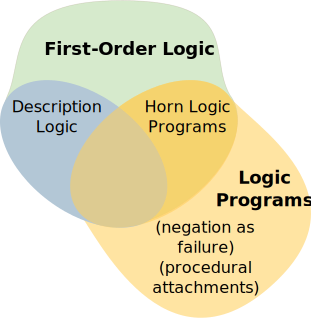
\includegraphics[width=0.6\columnwidth]{typology/expressive_overlap_dl_horn.pdf}
    \caption{expressiveness overlap of Description Logics and logic programs
    based on Horn clauses, taken from~\cite{Grosof2003}}
    \label{fig|overlap_dl_horn}
\end{figure}

Figure~\ref{fig|overlap_dl_horn} shows that the expressive power of description
logics and Horn clauses partially overlaps. In section~\ref{sect|reasoning} we
mention extensions to description logics based on rule systems to bring closer
the two approaches.

The relationships between expressive power and reasoning complexity that follow
has been extensively studied for Description Logics.
Zolin~\cite{ZolinDLComplexityNavigator} maintains a ``complexity navigator''
that allows to conveniently explore these relationships and indexes most of the
literature on that subject.

\subsubsection{Open World and Close World Assumptions}

The \emph{close world} (CWA) vs. \emph{open world} (OWA) assumption names a
modelling choice on the \emph{completeness} of a knowledge domain. In the close
world assumption, a proposition that can not be proven true is assumed to be
false (\emph{negation by failure}), while in the open world assumption, a
proposition may be considered either true, false or unknown.

This distinction is important in robotics were the robot may have to manipulate
concepts with only partial knowledge on them. For instance, let imagine a robot
that sees a bottle on a table, whose bottom is hidden by another object. The
robot can not prove that the bottle is indeed \emph{on} the table. A knowledge
representation system relying on the closed world assumption would then assume
the bottle is \emph{not} on the table ($\lnot R^{CWA}_{isOn}(bottle, table)$)
whereas with the open world assumption, the proposition $R^{OWA}_{isOn}(bottle,
table)$ would be undecided. Example in table~\ref{table|cwa-owa-example} provides
another example of consequences of the CWA/OWA choice on reasoning.

\begin{table}
    \begin{center}
    \begin{tabular}{ll}
    {\bf Action} & {\bf Part involved} \\
    \hline
    {\tt PickSoftly} & hand \\
    {\tt PickAndPlace} & arm, hand \\
    {\tt MoveArm} & arm \\
    \hline
    \end{tabular}
    \end{center}
    \caption{Assuming the question is: \emph{select actions that do not require
    to move the arm}, a CWA reasoner would return {\tt PickSoftly} whereas an
    OWA reasoner would not return anything if the {\tt PickSoftly} action is
    not explicitly said not to involve the arm.}
    \label{table|cwa-owa-example}
\end{table}

The OWL language is specifically known to assume an open world.  Domains
constrained with the closed world assumption lead to more tractable inference
problems, and allow for instance the use of logic languages like Prolog. Thus,
several approaches exists to \emph{locally close} a domain (\cf
Levesque~\cite{Levesque2008}, section 24.3.2 for a summary of those).

\subsubsection{Representation of uncertainty and likelihood}

Sources of uncertainty for a robot are two-fold: uncertainty \emph{intrinsic}
to facts (like \emph{``It may rain tomorrow''}), uncertainty caused by
imperfect perception of the world (\emph{``Is the bottle really on the
table?''}). Most logics do not account explicitly for uncertainty. It must be
either relied on specific logics (like Bayesian logics) or on extensions of
classical logics.

\subsubsection{Meta-cognition: knowledge on the knowledge}

As stated by Cox and Raja~\cite{Cox2007}, meta-cognition is composed of both
\emph{``meta-level control of cognitive activities and the introspective
monitoring of such activities to evaluate and to explain them"}.

A knowledge representation system endowed with \emph{meta-cognition} is not
only able to manipulate knowledge but also to exhibit and manipulate the
structure of its knowledge and the reasoning process. For instance, the ability
to explain a logical inconsistency in a KRS is a meta-cognitive function.
Sloman~\cite{Sloman2011} \fxfatal{...Sloman?}

At section~\ref{sect|introspection} below, we discuss the idea of
introspection.  Meta-cognition can be viewed as the technical facet of the
introspection in general.


%%%%%%%%%%
\subsection{How things are represented?}
\label{sect|higher-level-domain-representation}

\begin{scriptsize}
\begin{center}
\begin{tikzpicture}[taxonomy]
    \node [taxon] {\bf B. Representation}
            child {node [taxon] {{\bf B.5}. Memory}}
            child {node [taxon] {{\bf B.4}. Introspection}}
            child {node [taxon] {{\bf B.3}. Possible Worlds}}
            child {node [taxon] {{\bf B.2}. Context}}
            child {node [taxon] {{\bf B.1}. Roles}};
\end{tikzpicture}
\end{center}
\end{scriptsize}


\subsubsection{Role Representations}

Thematic roles

Spatio-Temporal Representations:

\paragraph{Representation of time}

As an agent acting at human-like time scale and dealing with temporal concepts
(like actions), a robot may want to represent, and possibly to reason, about
time. Time representation is split into two distinct abilities: representing
time points (both in the past -- which is roughly equivalent to assignment of
timestamps to events the robot perceives -- and in the future), and
representing \emph{passing time} (durations, timespans) like in \emph{``the
eggs will be cooked in 10 min''}.

\fxfatal{Discuss time chronicles~\cite{Ghallab1996}}
\fxfatal{Discuss Allen intervals}

We call a system that do not account for time (\ie that permanently lives in
present) \emph{atemporal}.

\paragraph{Representation of space}

\paragraph{Representation of events and actions}

\subsubsection{Context modeling}

\emph{Knowledge is contextualized information}\fxfatal{Find someone respectable
how said that :-)}: it is essential for the robot to associate the facts it
represents to a \emph{context}. The context carries the keys for the
interpretation of the information. It covers the \emph{domain of validity} of
the facts, the \emph{common-sense} knowledge required to fill the gaps in the
representation\fxfatal{give an example}, \fxfatal{What more?}.

\subsubsection{Possible-Worlds and representing what others know}
\label{sect|possible-worlds}

    
Linked to the context representation, but seen from another angle, knowledge
representation systems may provide explicit ways to model other point of view
on the world. This ability is often referred as the \emph{perspective taking}
ability.

\cite{Levesque2008}, p. 4

\subsubsection{Introspection: Who am I? What can I do?}
\label{sect|introspection}

\paragraph{Introspection}

Introspection is the ability to self-describe: what are my capabilities, what
is my state (performing some action, idling, etc.), what are my beliefs (\ie my
knowledge), what are my intentions and my plans?

Introspection must be distinguished from meta-cognition: While introspection
may require meta-cognition (for instance to be able to expose its internal
knowledge), it is not always mandatory. The current state of the robot can be
represented as a simple instantiation of a specific category (for instance, if
the robot give an object to the human, this state could be represented with the
triples \setstmt{robot performs action1, action1 isA Give}.

\paragraph{Modelling of the robot capabilities}

A particularly important aspect of introspection relates to the description of
its own capabilities: which sensors/actuators/computation services exist and
are currently available ?  While at a first level, these descriptions can be
static (\eg the robot has one laser scanner and two arms), at more advanced
levels, the description is updated and reflect the current (and possibly past
and future) state of the robot. Note that these description may also involve
geometric descriptions (a kinematic chain, the pose of a device, etc.) that may
be deported outside of the main knowledge base. Efforts trying to formalize,
maintain and expose the capabilities and state of a robot are not new (and
ground themselves in work and techniques for self-descriptive remote procedure
calls in computing science), but take a renewed importance with applications
for high-level multi-robot cooperation. Recent work in that direction
include~\cite{Kunze2011}.

\subsubsection{Memory}
\label{sect|memory}

Memory has been studied at length in the cognitive psychology and
neuropsychology communities: Atkinson and Shiffrin~\cite{Atkinson1968}
introduce the idea of \emph{short-term} and \emph{long-term} memory,
Anderson~\cite{Anderson1976} splits memory into \emph{declarative} (explicit)
and \emph{procedural} (implicit) memories, Tulving~\cite{Tulving1985} organizes
the concepts of \emph{procedural}, \emph{semantic} and \emph{episodic} memories
into a hierarchy. Short-term memory is refined with the concept of
\emph{working memory} by Baddeley~\cite{Baddeley2010}
(Figure~\ref{fig|memory_models}).

\begin{figure}
    \centering
    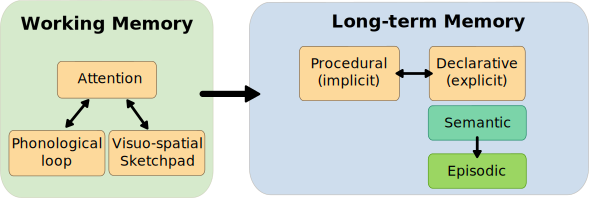
\includegraphics[width=0.9\columnwidth]{typology/memory_models.pdf}
    \caption{Overview of the main types of memories}
    \label{fig|memory_models}
\end{figure}

It worth emphasing that if memory is commonly associated to the process of
forgetting facts after a variable amount of \emph{time}, it covers actually
more mechanisms that are relevant to robotics, like selective remembering
triggered by a specific context or reinforcement learning.

Most knowledge representation systems offers some kind of memory as a pool of
facts that are not forgotten by the robot until it is halted (this memory is
often referred as a \emph{working memory}, but with a meaning unrelated to
Baddeley's definition). Some systems may propose persistent storages that allow
the robot knowledge to grow over time, while other may offer a larger range of
memory categories, like short term memory (that lasts for a couple of seconds)
or episodic memory (that allows the robot to selectively remember facts
associated to specific events).

In the larger field of cognitive architectures, the {\sc Soar}
architecture~\cite{Lehman2006} is one of those that tries to reproduce a
human-like memory organization.

%%%%%%%%%%
\subsection{Reasoning Techniques}
\label{sect|reasoning}

\begin{scriptsize}
\begin{center}
\begin{tikzpicture}[taxonomy]
    \node [taxon] {\bf C. Reasoning}
            child {node [taxon] {{\bf C.10}. Learning}}
            child {node [taxon] {{\bf C.9}. Naive physics}}
            child {node [taxon] {{\bf C.8}. Planning}}
            child {node [taxon] {{\bf C.7}. Prediction}}
            child {node [taxon] {{\bf C.6}. Presupposition}}
            child {node [taxon] {{\bf C.5}. Non-monotonicity}}
            child {node [taxon] {{\bf C.4}. Uncertainty}}
            child {node [taxon] {{\bf C.3}. Lazy evaluation}}
            child {node [taxon] {{\bf C.2}. Structural alteration}}
            child {node [taxon] {{\bf C.1}. Standard reasoning}};
\end{tikzpicture}
\end{center}
\end{scriptsize}


\subsubsection{Standard reasoning techniques}

Being based on logical languages to represent the knowledge, most of the
systems we survey allow various forms of \emph{reasoning}.

We call \emph{standard reasoning techniques} techniques based on logical
inference, using resolution algorithms like \emph{forward chaining},
\emph{backward chaining} or \emph{semantic tableaux}.

Main reasoning problems include \emph{concept satisfiability},
\emph{consistency checking} and \emph{instance checking}.

Concept satisfiability verifies if it is possible to find a non-empty
\emph{interpretation} of a concept (or an expression defining a concept) in the
knowledge model. For instance, the formula \concept{Plant} $\land$
\concept{isRed}, which defines the concept of red plants, is satisfiable in a
model \concept{KB} iff $\exists a, $ \concept{Plant}$(a) \land$
\concept{isRed}$(a)$, \ie if we can find at least one red plant $a$ in our
model.

Checking the consistency of a model is equivalent to checking the
satisfiability of each of the concept defined in the knowledge model.

Instance checking consists in verifying that an individual $a$ is an
interpretation of a concept (or concept expression) $C$ in the knowledge model.
A typical example would be that we are provided with an instance
\concept{object1} and we want to know if this object is a kind of
\concept{Bottle} or \concept{Glass}.

Reasoners can often provide other type of inferences, like:

\begin{itemize}
    \item class subsumption (similar to inheritance)

    \item reasoning on roles properties, including:
        \begin{itemize}
        \item entailments based on roles domain and range (for instance, if the
        domain of the role \concept{thinksOf} is known to be
        \concept{ThinkingAgent}, then \concept{thinksOf}$(a, b) \to
        $\concept{ThinkingAgent}$(a)$),

        \item universal, existential and cardinality constraints,

        \item property characteristics (inverse, symmetry, transitivity, etc.)

        \end{itemize}

    \item complex concept expressions like: \par \footnotesize \concept{Bottle}
    $\equiv$ \concept{Artifact} {\bf that} (\concept{hasShape} {\bf value}
    \concept{cylinderShape})\footnote{This example uses the \emph{Manchester
    syntax}, \url{http://www.w3.org/TR/owl2-manchester-syntax/}} \normalsize

    \item set operations like: \par \footnotesize \concept{Color} $\equiv \bigcup$ (\concept{blue}, \concept{green}, \concept{orange},
    \concept{black}, \ldots) \normalsize

\end{itemize}

\paragraph{Rule Languages}

As mentioned earlier, knowledge models based on description logics can be extended through rule languages.

Intersection of properties is an example of expression that can only be represented with rules: for instance, 

generic SWRL ({\em Semantic Web Rule Language}) rules like: \par
        \footnotesize \concept{looksAt(?agt, ?obj)} $\land$
        \concept{pointsAt(?agt,?obj)} \par $\Rightarrow$ \concept{focusesOn(?agt, ?obj)}
        \normalsize 


\subsubsection{Alteration of the knowledge structure}

The content of a knowledge base is often conveniently divided into a
\emph{structural part} that defines the conceptualisation of a domain in term
of vocabulary and relations within the concepts, and an \emph{instantiation} of
this structure into concrete entities.

The terms TBox and ABox are commonly found to describe this two different types of
statements in ontologies. TBox statements describe a system in terms of
controlled vocabularies, for example, a set of classes and properties. ABox are
TBox-compliant statements about that vocabulary.

All knowledge representation systems allow to modify the ABox, which can be
considered as the dynamic part of the knowledge base. It is however not always
possible to alter the TBox because not all reasoning systems can dynamically
take into account structural changes in the knowledge base.

Example of TBox alteration include modification of the taxonomy (like addition
or retractation of a \concept{subClassOf} relation), changes to the asserted
domain or range of a predicate, addition or retractation of rules.

Supporting TBox alteration has notable consequences on the learning
capabilities of the system: teaching general facts (\ie, facts at the level of
whole categories) like ``cars go on roads'' to a robot requires an alteration
of the TBox.

\subsubsection{Lazy evaluation}
\label{sect|lazy-evaluation}

\emph{Lazy evaluation} describes the ability for a KRS to delay active
knowledge acquisition or resoning operations until the value is actually
needed.

For instance, a system that computes the symbolic relative placement of two
objects only when this fact is required to answer a query would be said to
adopt a lazy evaluation strategy, whereas a system that computes {\it a priori}
such relations (and by consequence, carries out such computation for possibly
all known objects) would be said to use a \emph{strict evaluation} policy.

Lazy evaluation has an immediate impact on efficiency and scalability of the
system, and some problems may even be only tractable with a lazy evaluation
strategy (the relative placements of object is an example of combinatory
explosion in strict evaluation approaches, although this issue is mitigated in
real use-cases by heuristics that select a subset of objects to evaluate).

One downside is that the knowledge base never contains explicitly the complete
set of beliefs of the robot. This limits for instance the ability for the robot
to react to logical conditions that involves fact that are lazily evaluated
(``trigger a callback when object A is behind object B'' could be an example of
a event triggered by a logical condition).

\subsubsection{Reasoning with uncertainty}


\subsubsection{(Non) Monotonic Reasoning}

\emph{Monotonic reasoning} means that addition of new assertions to a knowledge base
can only extend the set of assertions that can be inferred, while a
\emph{non-monotonic} reasoning scheme may lead to retraction of facts.
McCarthy coined a famous example to illustrate the need of non-monotonic reasoning:

\begin{quotation}
Consider putting an axiom in a common sense database asserting that birds can
fly. Clearly the axiom must be qualified in some way since penguins, dead birds
and birds whose feet are encased in concrete can't fly. A careful construction
of the axiom might succeed in including the exceptions of penguins and dead
birds, but clearly we can think up as many additional exceptions like birds
with their feet encased in concrete as we like. Formalized non-monotonic
reasoning provides a way of saying that a bird can fly unless there
is an abnormal circumstance and reasoning that only the abnormal circumstances
whose existence follows from the facts being taken into account will be
considered.
\end{quotation}

Another important application of non-monotonic reasoning is representation of
change: for example, to make an omelette, you need to crack eggs and wipe them.
The eggs disappear and are replaced by an omelette:

\concept{Egg}$(a) \land $ \concept{Egg} $(b) \land $
\concept{MakeOmelette}$(a, b, c) \to \lnot $ \concept{Egg}$(a) \land \lnot $
\concept{Egg}$(b) \land $ \concept{Omelette}$(c)$

The insertion of the proposition \concept{MakeOmelette}$(a, b, c)$ leads to
retraction of other facts. This rule requires non-monotonic reasoning to be
applied.

\emph{Default logic} is one of the formal logic that account for representing
general truth and exceptions to it (for instance, \emph{tomatoes are red, in
general}). However, due to computational complexity of these model (most of
inferences in default logic are known to be $NP$-complete problem), classical
logics and most of the existing reasoners do not allow non-monotonic reasoning.
For instance, the SWRL rule language, usually associated to the OWL-DL ontology
language, do not allow non-monotonic reasoning (only so-called DL-safe rules
are allowed).

\fxfatal{Make clear 'who does not allow non-monotonic-reasoning': logics? rule
languages? reasoner?}

One important exception is the \emph{negation as failure} inference rule, as
implemented by {\sc Prolog} for instance, that allows for non-monotonicity
within the closed world assumption.

\fxfatal{Give here an example of non-monotonic reasoning with Prolog}
\fxwarning{Do we mention here Answer Set Programming?}

A monotonic system does not theoretically allow for knowledge retraction,
which is an important issue in the robotic context where the world model is
likely to be often altered.  However it is a practical issue only if the
reasoning process is \emph{continuous} during the whole robot's activity
lifespan. It is often possible to stop the reasoner, alter the knowledge, and
restart the inference process on a new domain.
\fxfatal{Rephrase to emphasize that when new evidences appear, it is anyway often a
good idea to restart the reasoner.}

\fxfatal{Mention that the 'change of world' issue can also be dealt with appropriate
time representation.}
\fxfatal{Mention that probabilistic reasoning lead to implicit non-monotonic reasoning}


\subsubsection{Presupposition Accommodation}
\label{sect|presupposition-accommodation}

\emph{Presupposition accommodation} is the ability for the system to
automatically create a context allowing to make sense of a proposition.

For instance, we can imagine a human telling a robot \emph{Please get me the
bottle that is behind you}. If the robot has not yet see what is behind it, it
needs to assume (and represents in its knowledge model) that a undefined bottle
can be found somewhere in the half of space behind it.

A knowledge representation system able to cope with presupposition
accommodation would be able to take into account this (usually under-defined)
information that is not grounded into perception for later inferences.

This ability to imagine a physically state of the world that is not actually
perceived can be seen as the converse of the grounding ability.

Note also that presupposition accommodation implies a bidirectional link of the
symbolic knowledge model with a geometric (or physical) model of the
environment. This article focuses on symbolic knowledge representation systems,
but we shall mention when a KRS explicitly provides support for presupposition
accommodation.

\subsubsection{Prediction, projection and diagnosis tasks}
\label{sect|prediction-projection}

Levesque~\cite{Levesque2008} distinguish two main tasks, the \emph{projection
task} and the \emph{legality task}.

\paragraph{Projection task}: determining whether or not some condition while
hold after a sequence of actions.

\paragraph{Legality task}: determining whether a sequence of action can be
performed starting in some initial state.

\paragraph{Diagnosis}: this corresponds to the ability to rewind on past events
in case of failure to provide possible explanation. This can be seen as the
temporal reverse of the projection task.

\subsubsection{Task Planning}
\label{sect|planning}

Making decision based on prediction

Symbolic task planning is the ability for a robot to select a sequence of
actions in order to reach a given final state. This capability is closely
related to the previously mentioned projection and legality tasks: for a robot
to plan, it must be able to build hypothetical states of the world that would
follow from the successive application of actions (prediction task), and at
each step, select possible, legal actions based on their pre-conditions
(legality task). As already mentioned, these tasks are highly non-monotonic.


Symbolic task planning in general is a large research
field\cite{Russell2009planning}. The so-called Classical Planning Problem,
first, is characterised by a unique known initial state, durationless
deterministic actions which can be taken only one at a time, and a single
agent. STRIPS and PDDL are amongst the commonly used languages for representing
such planning problems.

Planning with nondeterministic durationless actions with probabilities can be
represented as discrete-time \emph{Markov decision processes} (MDP), and when
full observability is replaced by partial observability, we deal with
\emph{partially observable Markov decision process} (POMDP).

\emph{Hierarchical Task Networks} (HTN) are another common formalism for
planning problems, where an initial set of tasks (\emph{High Level Tasks}, HLA)
is decomposed into either primitive actions or a new set of subtasks.

From the observation that the core reasoning techniques (back and forward
chaining) are shared between planners and reasoners used in knowledge
representation systems, task planning can be considered within the KRS.

It is however common to rely on external components dedicated to symbolic task
planning (in particular because of the non-monotonicity requirements) with a
tight link to the KRS for domain retreival and/or resulting plan storage.

%An extensive report on task modeling in OWL ontologies in appendix

\subsubsection{Physics-based reasoning}
\label{sect|physics}

As embodied entities, robots have to interact with physical entities.
\emph{Naive physics reasoning} covers all the everyday reasoning the humans
unconsciously perform, like taking into account gravity (``if I drop a ball, it
falls down'') or common physical properties of objects (``a glass may break if
dropped'', etc.). Many of the interactions with our everyday environments are
ruled by such laws that are difficult to exhaustively encode.

Some systems \cite{Kunze2011a} rely on external dedicated physics engine to
compute symbolic facts from on-demand physics simulation. This, however,
requires a tight integration between the symbolic model and a geometric model
that carries the geometries and physical properties of objects.

\subsubsection{Learning}
\label{sect|learning}

%%%%%%%%%%%%%%%%%
\subsection{Acquiring Knowledge}

\begin{scriptsize}
\begin{center}
\begin{tikzpicture}[taxonomy]
    \node [taxon] {\bf D. Acquisition}
            child {node [taxon] {{\bf D.4} Dynamic instantiation}}
            child {node [taxon] {{\bf D.3} Motivation}}
            child {node [taxon] {{\bf D.2} Grounding}}
            child {node [taxon] {{\bf D.1} Acquisition and fusion}};
\end{tikzpicture}
\end{center}
\end{scriptsize}

\subsubsection{Knowledge acquisition and modalities fusion}
\label{sect|knowledge-acquisition}

In the survey inclusion criteria, we have chosen to only consider robotic
systems that acquire knowledge by themselves, at runtime.

In our context, \emph{acquiring knowledge} means to build new logical
statements from data sources and to anchor them into the existing knowledge. We
consider three possible sources of data: proprioceptive/exteroceptive sensing,
interaction with other agents, humans or robots, and remote knowledge bases.
The acquisition process has generally two steps: the information acquisition by
itself, and the \emph{transformation} of the information into knowledge,
\emph{aligned} with the robot existing model (following our terminology for
information and knowledge, as discussed in the introduction).

It must be observed that knowledge acquisition is generally not done directly
in the knowledge representation system. External components (often aggregated
into knowledge acquisition \emph{pipelines}) are usually required to convert
percepts into symbolic facts and to ground them.

While we do not review in this article all these systems, the whole process of
knowledge acquisition is central in cognitive robotic architecture and the
design of knowledge representation systems can influence or be influenced by
the approach to knowledge acquisition.

In particular, complex robotic systems often require multi-modal perception
capabilities (for instance, a robot can only interpret an utterance like ``this
is a plate'' if it is able to understand gestures, understand natural language
and merge them in a timely manner). Multi-modal interpretation can take place
at various levels, but in many cases (especially if the modalities are of very
different natures, like in the example above) merging will require
symbolic-level reasoning. The KRS has a direct impact on the feasibility and
ease of such operations.

Let review shortly the three sub-categories of knowledge acquisition.

\begin{scriptsize}
\begin{center}
\begin{tikzpicture}[taxonomy]
    \node [taxon] {\bf D.1 Acquisition and fusion}
            child {node [taxon] {{\bf D.1.3} Linked Resources}}
            child {node [taxon] {{\bf D.1.2} Interaction}}
            child {node [taxon] {{\bf D.1.1} Sensing}};
\end{tikzpicture}
\end{center}
\end{scriptsize}

\paragraph{Sensing}

From the point of view of knowledge representation, the sensing capability can
be split into proprioceptive sensing (\ie, sensing of the robot own internal
state) and exteroceptive sensing (sensing of the robot environment). The
(physical) introspection capabilities of the robot relies on the former.

\fxwarning{What to say here?}

\paragraph{Interaction}

Interaction with other intelligent agents (humans or robots) is another
important source of knowledge acquisition. It relies obviously on some form of
sensing (from speech recognition to gesture recognition) but we distinguish it
from the previous section because \emph{interaction} implies a form of
communication. Communication is associated to specific functions
(figure~\ref{fig|communication-model}), and in particular, it implies a shared
\emph{context} (usually implicit) between interactors.


We distinguish between two main interaction channels: verbal and deictic.

\begin{scriptsize}
\begin{center}
\begin{tikzpicture}[taxonomy]
    \node [taxon] {\bf D.1.2 Interaction}
            child {node [taxon] {{\bf D.1.2.2} Deictic Interaction}}
            child {node [taxon] {{\bf D.1.2.1} Verbal Interaction}};
\end{tikzpicture}
\end{center}
\end{scriptsize}

\label{sect|nlp}

The field of verbal interaction processing for robots spans from pattern-based,
constrainted sentences recognition to natural, bidirectional, unconstrained
verbal communication. Kruijff et al. provides in~\cite{Kruijff2010} an
up-to-date survey of literature on situated human-robot dialogue, focusing on
formal representation systems, bi-directionality of the interaction and context
building.

Natural Language Processing (NLP) is a large research field by itself, and
while the robotic community may be lagging behind on many theoretical aspects,
it brings one important aspect: the embodiment. Because the interactors, both
the robot and the human, are establishing a communication within a shared
physical context, the verbal communication channel is complemented by deictic
channels, back channels and possibly shared physical experiences: a human can
show something to a robot, saying ``Give me this''. This is simply not possible
for a virtual agent.

Several of the knowledge representation systems we present have developed
specific built-in mechanisms or extensions to parse, ground and possibly
rebuild natural language.

Deictic (used in the literal meaning of ``display, demonstration, reference'')
interaction is also an established field of research in human-robot
interaction. Common deictic forms of communication include attentional focus
(via face and gaze tracking) and joint attention, pointing, emotional
expressions (based on face expressions, postures, emotional gestures).

Like other knowledge acquisition modalities, the recognition and interpretation
of deictic communication is rarely directly included in a KRS, but, as
previously mentioned, the symbolic representation of such communication acts is
relevant and important to achieve successful multi-modal interactions.

\paragraph{Linked Knowledge Resources}
\label{sect|lod}

Robots, and in particular service robots, can access (with sometimes some
security-related constraints) the World Wide Web and remote knowledge stores.

The current shift towards the Semantic Web (\ie structured, annotated data that
are easily machine-processable) makes increasingly easy to have robots to reuse
autonomously this knowledge. The DBPedia project, for instance, illustrates
well the tendency: it provides an automatically generated RDF version of the
Wikipedia encyclopedia.

In its current state, the relevance of the DBPedia project in our context is
however limited: the triples that are extracted are mostly ``mechanical'' (like
the categories of a term, or factual informations extracted from Wikipedia's
InfoBox), and the vast majority of the knowledge actually contained in the
encyclopedia pages remains out of reach of automated parsers. Efforts like {\sc
ReVerb}~\cite{Fader2011} work however at automatic extraction of triples by
examining subject-verb-object relations in plain text.

Another notable project that seeks at providing large amount of
machine-friendly common-sense knowledge is the MIT's OpenMind
project~\cite{Singh2002}. The project is designed to let the general public
easily add common-sense statements in semi-controlled natural language, that is
then processed to a publicly available ontology.

An other approach that is easier at short-term to let robots remotely access
knowledge repositories consists is building robot-specific shared repositories,
with declarative and/or procedural (\ie, plan library) knowledge. The
RoboEarth~\cite{Waibel2011} project is an example of such an effort.

\subsubsection{Grounding/anchoring strategies}
\label{sect|grounding}

\emph{Grounding} (also called \emph{anchoring} when specifically referring to
building links between \emph{percepts} and \emph{physical
objects}~\cite{Coradeschi2003}) is the task consisting in building and
maintaining a bi-directional link between sub-symbolic representations (sensors
data, low-level actuation) and symbolic representations that can be
manipulated and reasoned about~\cite{Harnad1990}.

Being embodied entities with interaction with other embodied entities as a
fundamental requirement, robots and robotic is deeply concerned by the
grounding issue.

Being actually implemented on real service robots, all the symbolic knowledge
representation systems that we review in this study have some kind of grounding
process. Numerous approaches exist, like amodal
\emph{proxies}~\cite{Jacobsson2008}, grounded amodal
representations~\cite{Alami2011, Mavridis2006}, semantic maps
(Figure~\ref{fig|semanticmap}, \cite{Nuechter2008, Galindo2008,Blodow2011}) or
affordance-based planing and object classification~\cite{Lorken2008,
Varadarajan2011}.

\begin{figure}
    \centering
    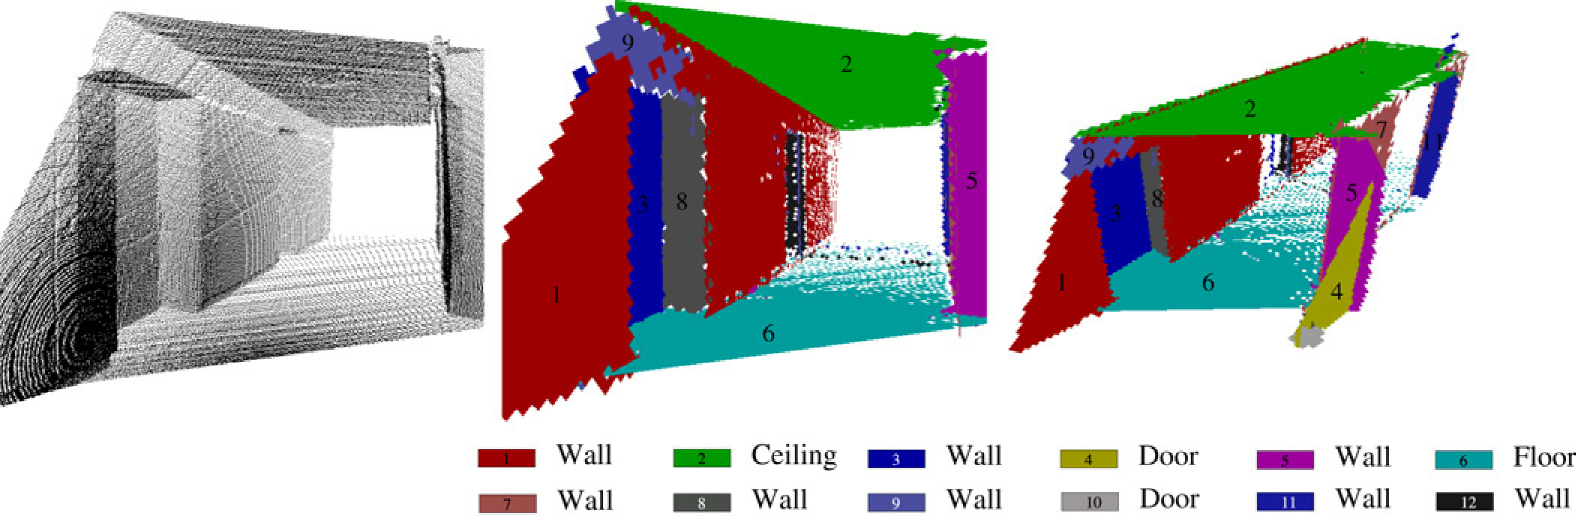
\includegraphics[width=0.9\columnwidth]{typology/semanticmaps_hertzberg.png}
    \caption{Example of a semantic map, taken from~\cite{Nuechter2008}.}
    \label{fig|semanticmap}
\end{figure}

\subsubsection{Intrinsic Motivation}

\cite{Oudeyer2007} -> page 2 gives a detailled account of psychological grounds.
Curiosity, Pro-active behaviour...

\subsubsection{Dynamic instantiation}
\label{sect|new-instances}
Ability to automatically create new object instances

%%%%%%%%%%%%%%%%%
\subsection{Practical Integration in Robotic Architectures}
\label{sect|integration-robot}

\begin{scriptsize}
\begin{center}
\begin{tikzpicture}[taxonomy]
    \node [taxon] {\bf E. Integration}
            child {node [taxon] {{\bf D.4} Performances}}
            child {node [taxon] {{\bf D.3} Monitoring}}
            child {node [taxon] {{\bf D.2} Executive layers}}
            child {node [taxon] {{\bf D.1} Sensori-motor}};
\end{tikzpicture}
\end{center}
\end{scriptsize}


Knowledge representation systems do not mean anything to robots if they are
considered in isolation. This section proposes categories of features related
to the integration of the KRS into a larger software architecture that includes
perception routines, decision-making processes and actuation control.

We also mention some practical aspects of a real-world system, like
performances and monitoring tools that come along with the KRS.

\subsubsection{Integration with sensori-motor layers}
\label{sect|integration-sensorimotor}

We have previously discussed (section~\ref{sect|grounding}) the principles of
the grounding process that aims at establishing and maintaining a connection
between percepts (and to a lesser extend, low-level actions) and symbols.

While every real-world cognitive robot need some kind of grounding, the actual
implementations lead to very different information flows.

The systems can be roughly split into two classes: \emph{passive} knowledge
repositories that process symbolic facts produced by lower-level sensori-motor
layers (\emph{push} flow); \emph{active} knowledge managers that directly query
(possibly by polling or on-demand) low-level layers.

This macroscopic distinction is however mostly a matter of defining the
frontiers of the KRS: some systems like KnowRob~\cite{Tenorth2009a} encompass
geometric reasoning layers that would be considered as external by other
systems like ORO~\cite{Lemaignan2010} that focus on the symbolic fact storage
and rely on a ecosystem of independent modules to provide and consume symbolic
knowledge.

\fxwarning{Some archi with the ability to ``listen'' to the robot internal
structures -> which ones?}

Other systems do not fit either in such a partition between active and passive
systems because they do not stand as independent modules but exist as diffuse,
\emph{ubiquitous} knowledge manipulation system~\cite{Jacobsson2008}, for
instance because they are primarily language~\cite{Ferrein2008, Sabri2011}.

\subsubsection{Integration with executive layers}
\label{sect|integration-executive-layers}

Conversely, the knowledge management module need a tight integration with the
decision-making processes. As for the integration with sensori-motor
layers, the borders of the KRS can be fuzzy and vary from one architecture to
another: many consider symbolic task planning as an integral role of the KRS,
while other have dedicated extensions for planning, some integrate learning as
an on-the-flight process that is part of the KRS, others as an independent
deliberative process, etc.

The actual integration techniques vary also widely, from language extensions
(like the integration of CRAM~\cite{Beetz2010} with KnowRob) and client-server
architectures, to event-driven models (SHARY and ORO~\cite{Alami2011}). Choices
at this level have notable consequences on the whole design of the upper
control architecture of the robot, in particular regarding its modularity and
the ease of addition of new components.

\subsubsection{Monitoring and debugging}
\label{sect|debugging}

It is common to have knowledge representation systems at the heart of a
cognitive robotic architecture, and therefore KRS are easily ``burried'' in the
system.

At the same time, the symbolic model often provides a valuable synthetic view
on the whole state of the robot, furthermore easily understandable by the human
developer (the fact \stmt{human1 isSitting true} is easier to interpret than
the suite of relative coordinates of each joints of the human skeleton, as
provided by the human tracker, for instance).

That is the reason why having at hand good tools to trace and visualize at
run-time the evolution of the knowledge structure and contents, as well as
post-processing tools that can be run on the trace to precisely analyze the
cognitive behaviour of the robot, is useful.

\subsubsection{Evaluation of performances}
\label{sect|performances}


Benchmarks of symbolic systems for robots are hard to conduct for
several reasons: identifying good metrics for robotic experiments in general is
difficult because of the complex interactions between tenth of modules running
in parallel, and isolating one specific component is difficult.
Also, knowledge representation systems are often tightly coupled to
the other modules, and the lack of standard API for knowledge services
makes it especially hard to switch between KRS to compare them. Finally, because
service robots are design to act in rich, dynamic environments, possibly with
humans, building repeatable experiments is challenging.

\begin{scriptsize}
\begin{center}
\begin{tikzpicture}[taxonomy]
    \node [taxon] {\bf D.5 Performance \\Evaluation}
            child {node [taxon] {{\bf D.5.2} Cognitive Performances}}
            child {node [taxon] {{\bf D.5.1} Raw Performances}};
 \end{tikzpicture}
\end{center}
\end{scriptsize}


\paragraph{Raw Performances} The \emph{raw performance} is evaluated on
quantitative benchmarks. The main metric is the \emph{scalability}
$\mathcal{S}^{KRS}$ of the system with the size of the knowledge base
$\sigma=|\Delta^{\mathcal{I}}|$  (in term of atoms or statements).

We call \emph{relaxation time} $\mathcal{R}^{\mathcal{M}}$ the (averaged) time
required by the system after a model modification of type $\mathcal{M}$ before
being available for further interaction, and \emph{query time}
$\mathcal{Q}^{\mathcal{M}'}$ the (averaged) time to execute a query of
complexity $\mathcal{M}'$ on the KRS. The type $\mathcal{M}$ of model
alteration is either an ABox modification (addition/removal of an instance) or
a TBox alteration (addition/removal of a class, a class restriction or a rule).
Query complexity $\mathcal{M}'$ is...\fxwarning{find references}.

\emph{Temporal scalability} is defined in term of the nature of the function
$f^{\mathcal{M}, \mathcal{M}'}(\sigma) = \mathcal{R}^{\mathcal{M}}(\sigma) +
\mathcal{Q}^{\mathcal{M}'}(\sigma)$ (\ie the relation of the relaxation time
and query time to the knowledge base size). \emph{Space scalability} is the
relation of memory consumption to the size. The scalability is tightly coupled
to the expressiveness of the underlying knowledge model, which need to be known
for the scalability measurement to be meaningful.

Note that robotic applications may have a knowledge base size relatively small
compared to the complexity of its TBox. In that case the relaxation and query
times for a constant, average knowledge size $\sigma$ may be more relevant as a
metric for KRS raw performance.

Because of coupling and repeatability issues we have mentioned, raw
performances of KRS are often benchmarked with synthetic datasets (which leads
to issues: how to assess the meaningfulness of the performance of a reasoner on
an artificial ontology?~\cite{Bail2010}) or toy experiments~\cite{Chong2009}
that do not always model the whole complexity of real-world application.

\paragraph{Cognitive Performances} While evaluating the raw performances of
knowledge representation systems in a relevant manner may be difficult, the cognitive
performances of the robot as a whole can be also evaluated through
``classical'' tests from the psychology (like False-Belief
experiments~\cite{Leslie2000} or the Token test~\cite{DiSimoni1978}).

However, the performance evaluation of current tools is mostly qualitative and
scenario-specific (``did my system do the job for my task?''), and amongst the
surveyed KRS, only few systems proposes an evaluation of their performances
that could be compared to other system.

%%%%%%%%%%%%%%%%%%%%%%%%%%
\subsection{Knowledge instantiation}

\begin{scriptsize}
\begin{center}
\begin{tikzpicture}[taxonomy]
    \node [taxon] {\bf F. Knowledge instantiation}
            child {node [taxon] {{\bf F.5} Self-Knowledge}}
            child {node [taxon] {{\bf F.4} Metrics}}
            child {node [taxon] {{\bf F.3} Granularity}}
            child {node [taxon] {{\bf F.2} Common-sense and Alignement}}
            child {node [taxon] {{\bf F.1} Design Strategy}};
 \end{tikzpicture}
\end{center}
\end{scriptsize}

This last branch of our taxonomy looks at the actual \emph{content} of the
knowledge base: the knowledge instantiation. Here, \emph{instantiation} does
not only refer to the instantiation of the knowledge structure (what we have
called the ABox), but also includes the knowledge structure itself (the TBox).

While we have previously mentioned features of knowledge representation system
that enable the robot to fill its knowledge base with content and alter the
knowledge structure, most of the systems also come with a certain amount of
initial knowledge that often includes \emph{common-sense} knowledge (\ie facts
that widely known to humans, and hence often implicit: ``to put a cake in the
oven, one must first open the oven's door'').

The design strategy, the choice to rely on common-sense knowledge or not, the
reuse of standard ontologies, the quantity of {\it a priori} knowledge are many
parameters that lead to different knowledge models.

\subsubsection{Design Strategy}

Ontology engineering has grown into a research field of its own, covering
formalized methodologies for ontology creation, reuse, modularisation, etc.

The creation

Two main approaches are common in the cognitive robotic community:
\emph{top-down} design and \emph{bottom-up}.

\subsubsection{Common-sense and alignment with Standard Upper-ontologies}

At section~\ref{sect|lod} we have presented how remote knowledge bases are a
valuable source of knowledge, including common-sense knowledge, that robot can
extract.

\subsubsection{Granularity}

The knowledge \emph{granularity} qualifies the level of details or refinement
of the knowledge stored.

...

The storage of literal values is a particular case: while knowledge
representation systems have been considered until now mostly as symbolic
systems, they can often represent literal values (in particular, numerical
values) as well.

Depending on the representation language, literal values can be naturally
represented and processed (common case in logic programming language) or not
(storing numerical value, let alone matrices, in OWL is cumbersome).

\subsubsection{Metrics}

Qualitative and quantitative metrics give an insight on the size and
expressive complexity of ontologies.

Table~\ref{table|upper_onto_metrics} gives such metrics for four major
upper-ontologies commonly used in the semantic Web community (taken
from~\cite{Mascardi2007} and the projects' respective websites).


\begin{table}
\begin{center}

\begin{tabular}{llllll}
\toprule
{\bf Project} & {\bf Terms} & {\bf Assertions} \\
\midrule
Cyc & > 300 000 & > 3 000 000 & \\
YAGO & > 10 000 000 & > 120 000 000 \\
SUMO & 20 000 & 60 000 \\
DBPedia (for English) & 1 840 000 & 385 000 000\\
OpenMind Common Sense (for English) & & 1 000 000\\
\bottomrule

\end{tabular}
\end{center}
\caption{Selection of metrics for the major upper-ontologies.}
\label{table|upper_onto_metrics}
\end{table}



\subsubsection{Self-Knowledge}

``Self-knowledge'' is the term used in psychology to describe the knowledge
that an individual has, acquires or infers about itself through its
experiences. It answers the question ``What am I like?''.

For a robot to have at its disposal self-knowledge is closely link to the
introspective capability that we have previously mentioned
(section~\ref{sect|introspection})


%%%%%%%%%%%%%%%%%%%%%%%%%%%%%%%%%%%%%%%%%%%%%%%%%%%%%%%%%%%%%%%%%%%%%%%%%%%%%%%%%%%%%%%%%%%
\section{Surveyed systems}
\label{sect|surveyed-systems}

Table \ref{table|surveyed-systems} presents the eight knowledge representation
systems surveyed in this article.

This section briefly presents each of them.

\begin{landscape}
\begin{table}\footnotesize
\begin{center}

\begin{tabular}{p{2.2cm}p{1.6cm}p{4cm}lp{2.4cm}p{3.4cm}p{2.8cm}p{1.5cm}}
\toprule
{\bf Project} & {\bf Category} & {\bf Authors (Institution)} & {\bf Project homepage} & {\bf Programming language} & {\bf Knowledge model/Logical Formalism} & {\bf Reasoner} & Main reference \\
\midrule
{\sc KnowRob} & KRS & Tenorth, Beetz \par (TU Munich) & \url{ias.in.tum.de/kb/wiki} & {\sc Prolog} & {\sc Prolog} + OWL-DL & Custom \par ({\sc Prolog}) & \cite{Tenorth2009a} \\
ORO & KRS & Lemaignan, Alami \par (LAAS-CNRS) & \url{oro.openrobots.org} & {\sc Java} & OWL-DL ({\sc Jena}) & {\sc Pellet} & \cite{Lemaignan2010} \\
PEIS KR\&R & KRS & Daoutis, Coradeshi, Loutfi, Saffiotti \par (Örebro Univ.) & \url{www.aass.oru.se/~peis} & {\sc C}, {\sc CycL} & CycL (1st and 2nd order logics, modal logics) & & \cite{Daoutis2009} \\
CAST Proxies & Ubiquitous & Wyatt, Hawes, Jacobsson, Kruijff (Brimingham Univ., DFKI Saarbrücken) & & & Amodal proxies & & \cite{Jacobsson2008} \\
NKRL & Language & Zarri et al. \par (Paris Est Créteil Univ.) & & NKRL & & & \cite{Sabri2011} \\
GSM & KRS & Mavridis, Roy \par (MIT MediaLab) & & ? & & & \cite{Mavridis2006} \\
OMRKF & KRS & Suh et al. \par (Hanyang Univ.) & \url{incorl.hanyang.ac.kr/xe} & ? & Horn Clauses & ? & \cite{Suh2007} \\
Ke Jia Project & KRS & Chen et al. \par (Univ. of Science and Technology of China) & \url{www.wrighteagle.org/en} & ASP & ASP & ASP & \cite{Chen2010} \\
ARMAR/Tapas & KRS & Holzapfel, Waibel \par (Karlsruhe TH) & & ? & TFS (Typed Feature Structures) & & \cite{Holzapfel2008}\\
Golog & Language & Levesque (Toronto Univ.) & & {\sc Prolog} & & & \\
OBOC & KRS & Mendoza & & & & & \cite{Mendoza2005} \\
% & & Varadarajan, Vincze \par (TU Wien) & & & & & \cite{Varadarajan2011} \\ % -> affordances, but no implementation on a robot
% & & Kaelbling, Lozano-Pérez \par (MIT CSAIL) & & & & & \cite{Kaelbling2011} \\ % -> mostly planning under uncertainty
% & & Hertzberg (Osnabrück Univ.) \\ % -> affordances, semantic mapping
% (based on {\sc KnowRob} & & (JSK) \\

\bottomrule

\end{tabular}
\end{center}

\caption{List of surveyed systems. Projects are listed by category (\emph{KRS}
for systems that are explicit knowledge representation and reasoning modules,
\emph{Ubiquitous} for systems where knowledge processing is fully distributed,
\emph{Language} for languages used as KRS on robots), then names.}

\label{table|surveyed-systems}
\end{table}
\end{landscape}

\fxfatal{Bielefeld -> could not find much...}
\fxfatal{Kollar/Tellex -> really focusing on the natural language grounding}

\subsection{KnowRob}
\label{sect|knowrob}

\subsection{ORO}
\label{sect|oro}

\subsection{PEIS KR\&R}
\label{sect|peis-ecology}


{\sc PEIS Ecology}~\cite{Saffiotti2005} is a software \emph{ecosystem} that aim to binds autonomous
robotics with ambient intelligence (network of sensors). \emph{PEIS} stands for
\emph{Physically Embedded Intelligent System}: every robots or intelligent
device in the environment is abstracted as a PEIS.

Each PEIS physical component is running a \emph{PEIS Kernel} instance. Communication
between instance relies on a custom P2P communication protocol.

The PEIS architecture allows for adding new abilities through software components sharing the common \emph{tuple space}.

We survey here the semantic layer~\cite{Daoutis2009}, referred as \emph{PEIS KR\&R}, that includes symbolic representation and reasoning.

% More in details:
% - object identification based on viewpoint independent SIFT features
% - formalized anchoring system that explicitly match percieved attributes to predicates
% - Cyc predicates
% - ground 12 colors, based on a paper on color perception. Could be useful for us.
% - idem, they cite a paper on what spatial relations to compute
% - location of objects based on a previously provided semantic map (but not much on this semantic map)
% - two "memories": the robot memory stores the current list of percieved objects ; the archive memory stores what is not percieved anymore
% - uses directly Cyc (ie, 250 000 common sense concepts...), via CycL language -> 2nd and higher order logics (quantification over predicates, functions, etc)
% Remark: using 2nd order logic (ie meta statements), it would be easy to store the knowledge of each agent
% - disambiguation in concept name by asking human to decide amongst all concepts known by Cyc
% - template based natural language
% - experiment conducted in a "smart" indoor environmement + simple robot

\paragraph{Knowledge model} The PEIS Knowledge representation system relies on
the {\sc ResearchCyc} and {\sc CycL} language to represent knowledge. The {\sc CycL} language
allows to represent first order logic sentences and has extensions for modal logics and higher order logics.

\fxfatal{Is modal logics and higher order logics actually used in PEIS?} 

As a system relying on {\sc CycL}, contexts can be expressed as
\emph{microtheories}: the truth or falsity of a set of statement depends of the
\emph{microtheory} in which these statements are evaluated.

\fxfatal{OWA/CWA?}

\begin{figure}
	\centering
	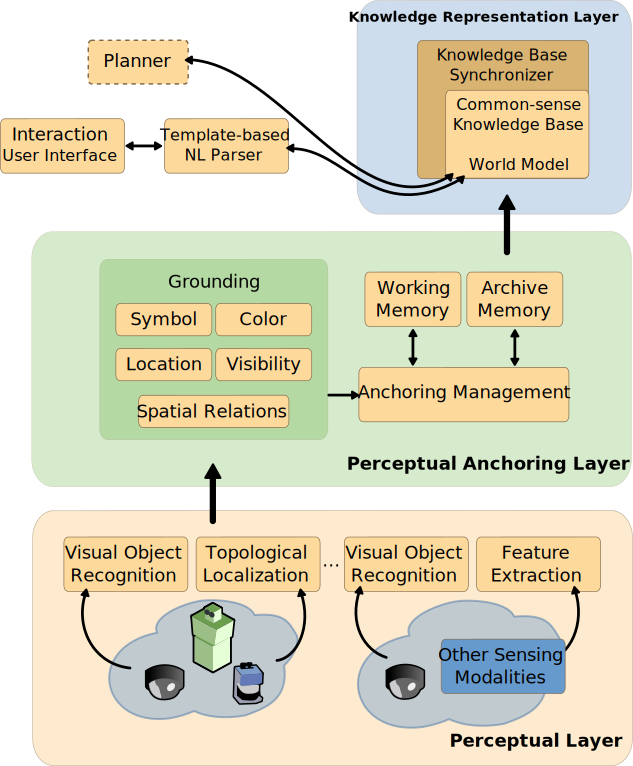
\includegraphics[width=0.9\columnwidth]{stateofart/peis-architecture.pdf}
	\caption{The PEIS knowledge representation system, taken from~\cite{Daoutis2009}}
	\label{fig|peis-archi}
\end{figure}

The PEIS KR\&R system is deeply integrated to the general PEIS Ecology
\emph{smart} environment. Figure~\ref{fig|peis-archi} gives an overview of the
interactions between PEIS knowledge processing layers.

\paragraph{Knowledge Acquisition} The primary source for knowledge acquisition
is perception.  The PEIS ecosystem provides a SIFT-based object recognizer used
in conjunction with ceiling cameras for object localization.  Other perceptual
modalities are available (like human tracking, ambient environment monitoring).

A template-based natural language parsing system may also be used to add new
assertions to the system.

The system can ask the human for help to disambiguate between concept names.

\paragraph{Anchoring} Daoutis et al. formalize the issue of anchoring as
finding a \emph{predicate grounding relation} $g \subseteq \mathcal{P} \times
\Phi \times D(\Phi)$, where $\mathcal{P}$ is a set of predicate symbols, $\Phi$
a set of percept's attributes, and $D(\Phi)$ the domain of these attributes.

In the current implementation, object category (returned by the SIFT
classifier), color, location, spatial relations (both topological -- \emph{at},
\emph{near} -- and relative to the robot -- \emph{left}, \emph{behind}, etc.)
and visibility are the five classes of extracted attributes.

\paragraph{Integration in the robot architecture}
\label{sect|peis-integration}

The PEIS framework offers through the \emph{PEIS middleware} a practical way to
insert a new component into the shared \emph{tuple space}.  Thus, the KR\&R
module can be seamlessly integrated into the PEIS ecosystem.

\subsubsection{Notable experiments}
\label{sect|peis-expe}

\subsection{NKRL}
\label{sect|nkrl}

\emph{NKRL} stands for \emph{Narrative Knowledge Representation Language}.
While this language is developed since a long time by Zarri~\cite{Zarri1997,
Zarri2008}, recent research direction include application to the robotic
field~\cite{Sabri2011}. NKRL is not {\it per-se} a knowledge representation
system, as it is primarily a language. However, it is used as the
representation and reasoning mechanism for robots by Sabri et al.

\subsubsection{Intrinsic language features}
\label{sect|nkrl-intrinsic-features}

\paragraph{Expressiveness}

\subsubsection{Integration with physical world and in the robot architecture}
\label{sect|nkrl-integration}

...seem to be mostly WIP...


\subsection{CAST Knowledge model}
\label{sect|cast}

CAS (\emph{CoSy Architecture Schema}) Toolkit~\cite{Hawes2007} is a
comprehensive toolkit aimed at building cognitive architectures for robots
through a set of interconnected SAs (\emph{subarchitectures}). The CAS does not
expose a central knowledge base as seen in previous works. It instead
represents knowledge as unrooted \emph{proxies}. Those proxies are formally
defined in \cite{Jacobsson2008} as $p= \langle F_p, u_p \rangle$ where $F_p$ is
a set of instantiated features (like $\phi^{Colour}_{red}$) and $u_p$ a
\emph{proxies union} that form an equivalence class corresponding to one
entity.

A union of proxies forms a global amodal representation of an entity, that can
be explicitly shared and manipulated. Being not centralized, the knowledge
model can be qualified of \emph{ubiquitous}. Furthermore, knowledge source in
the CAS architecture is tightly bound to the on-line grounding process (be it
grounded in perception or in dialogue). While nothing seems to prevent it, no
{\it a priori} knowledge (including common-sense knowledge) is used.

Knowledge sharing is ensured by the event mechanism of CAST: modules can
monitor proxies for alteration by other modules. Jacobsson et al. mention how
this can apply to reinforcement learning: the vision module creates a proxy for
an orange object. This proxy get monitored by a learning module. In parallel,
the proxy is bound to an union by the natural language understanding module
that add new a feature like \emph{"this object is a fruit"}. The learning
module is called back, and can add this new information to its model.

In the presented implementation, the CAST knowledge model does no allow for
effectively representing actions or temporal information.\fxfatal{What about reasoning? can they retrieve for example 'all proxies for colorful objects'?}

\subsection{GSM}
\label{sect|gsm}

GSM (for \emph{Grounded Situation Model})~\cite{Mavridis2006} is a knowledge
representation system primarily built to ``facilitate cross-modal
interoperability'',  especially in the context of verbal interaction with a
robot.

Unlike most of the previously presented systems, GSM does not rely on any
formal language but rather on a layered data structure (Figure~\ref{fig|gsm})
that organizes the surrounding world into agents and relations between agents.
Each agent (any animate or inanimate object) is attached to a physical model (made
of \emph{body parts} that have properties like their position, color, etc.) and
a mental model (which is a recursively embedded GSM, thus allowing a sort of
theory of mind).

\begin{figure}
    \centering
    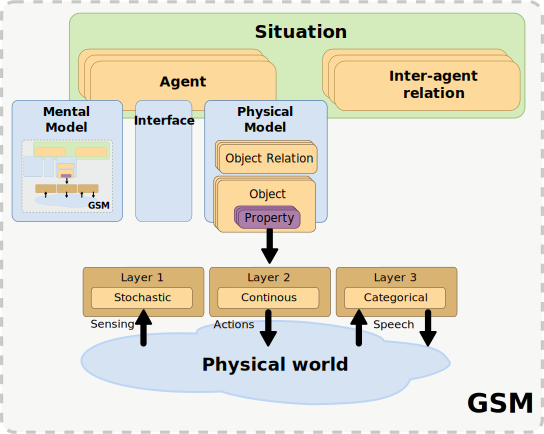
\includegraphics[width=0.9\columnwidth]{stateofart/gsm.pdf}

    \caption{Simplified hierarchical structure of the Grounded Situation Model,
    based on~\cite{Mavridis2006}}

    \label{fig|gsm}
\end{figure}

Properties are represented in three layers: a stochastic representation, close
to sensory percepts, a \emph{continuous single-valued} encoding of the
stochastic model, and a discrete, categorical model.

One notable feature of GSM is the \emph{bidirectionality} of the grounding
process: not only sensor percepts are abstracted into categories suitable for
human conversation, but human utterance (like ``There is a red ball in the
center of the table'') can also be turned into property descriptions. This
basically enable the knowledge representation system of the robot to
\emph{imagine} entities.

GSM also features several strategies for managing time and events.
\emph{Moments} are created by storing timestamped snap-shots of GSM, and
\emph{event classifiers} allow to define and detect events.

\paragraph{Experiments} GSM has mostly been tested on table-top manipulation
and interaction tasks (a ``conversational helping hand'' as stated by the
authors) realized on a 7-DOF arm equipped with force feedback, cameras for blob
tracking and speech recognition (Sphinx4). Mavridis and Roy provide in addition
an in-depth analysis of the performance of GSM by the mean of a standard
psycholinguistic test, the \emph{Token test}~\cite{DiSimoni1978}.

\subsection{OMRKF}
\label{sect|omrkf}

The Ontology-based Multi-layered Robot Knowledge Framework~\cite{Suh2007}
(OMRKF) is a knowledge representation system based on four inter-related
\emph{classes} of knowledge (Figure~\ref{fig|omrkf}). It proposes a layered
approach to knowledge representation that allows to integrate the grounding
process to the knowledge representation process. OMRKF knowledge model is
implemented with Horn clauses.

\begin{figure}
    \centering
    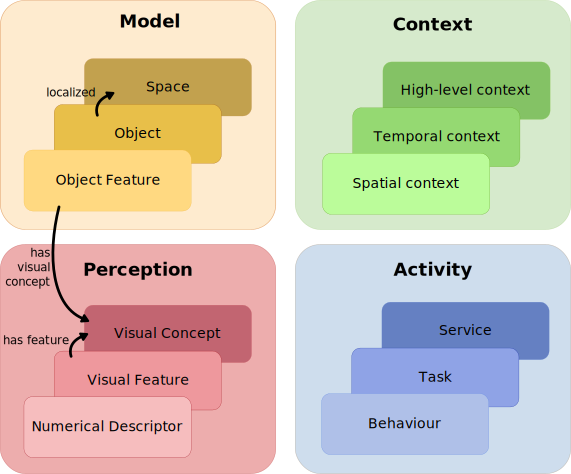
\includegraphics[width=0.8\columnwidth]{stateofart/omrkf.pdf}

    \caption{OMRKF organizes knowledge into four \emph{classes}, each composed
    of three \emph{levels}. The figure shows some examples of link between
    knowledge classes and knowledge levels. Based on~\ref{Suh2007}.}

    \label{fig|omrkf}
\end{figure}

Each level of knowledge is build as three stages of ontological realization: a
\emph{meta-concept} (the level itself, like ``temporal context'', ``behaviour''
or ``object feature'', a taxonomy of concepts inside this level (for instance
$cup : Object \sqsubseteq tableware : Object$) and an instantiation of the
taxonomy ($cup1 : cup$).

Environment is represented in OMRKF in the $space : Model$ knowledge level as a
classical three layers mapping (metric, topological and semantic maps). Objects
(in $object : Model$) are localized in $space : Model$ through Voronoi nodes.

The knowledge class $Context$ proposes an explicit statement of spatial context
(mostly geometric relations between objects), temporal context and a more
general \emph{high-level} context, inferred from spatial and temporal contexts.

Finally, the $Activity$ knowledge class store compound actions in a HTN-like
structure, exploited at run-time by a planner.

\paragraph{Experiments} Experiments conducted with OMRKF include finding
kitchen objects and reporting about their state to a human.  This experiment
also shows how OMRKF can deal with objects only partially matched by their
descriptor by introducing a $candidate()$ function.

\subsection{Ke Jia Project}
\label{sect|kejia}

The Ke Jia project~\cite{Chen2010} integrates on a mobile platform a knowledge
representation language with natural language processing, task planing and
motion planing.

Knowledge representation relies on \emph{Action Language C}, itself based on
\emph{Answer Set Programming} (ASP)~\cite{Gelfond2008}. These languages, that
are syntactically close to Prolog, are based on \emph{stable models} of logic
programs, and support non-monotonic reasoning. Default and non-monotonic
reasoning has been especially researched within the Ke Jia project for symbolic
task planing~\cite{Ji2011} and underspecified natural language processing.

Amongst other features, the natural language processing capabilities of the
system support acquisition of new logical rules at run-time.

\paragraph{Experiments} The Ke Jia robot has been demonstrated in several tasks
involving human-robot interaction with natural language. These tasks include a
task with multiple \emph{pick \& carry} that are globally optimized, naive
physics reasoning via taught rules or more complex scenarii with the robot
delivering drinks, taking into account changing and mutually exclusive
preferences of users.

\subsection{ARMAR/Tapas}

{\sc Tapas} is the name of the knowledge representation system and dialogue
manager found on the ARMARIII robot~\cite{Holzapfel2008}.

Knowledge in {\sc Tapas} exists as procedural knowledge (plans) and declarative
knowledge. The later is split into \emph{lexical knowledge}, \emph{semantic
knowledge} and a database of identified objects (with their properties). The
\emph{lexical knowledge} contains lexical and grammatical informations about
the objects. The \emph{semantic knowledge} is organized into an ontology
relying on \emph{typed feature structures} (TFS,~\cite{Carpenter1992}, a
formalism originating from the computational linguistics community, and a
superset of first-order logic).

{\sc Tapas} has a strong focus on natural language grounding. It proceeds by
generating grammars from properties represented in the ontology to parse and
understand dialogue.

Another focus is put on handling unknown words and objects. {\sc Tapas}
provides routines to recognize unknown entities, and propose and interactive
and iterative verbal process to categorize (including adding new categories)
those new concepts.

%%%%%%%%%% Underlying knowledge model table %%%%%%%%
\begin{table}
\begin{center}

\begin{tabular}{lp{4cm}}
\toprule
{\bf Project} & {\bf Common-sense \par knowledge source} \\
\midrule
{\sc KnowRob} & {\sc OpenCyc}, processed web content, custom OWL-DL ontology \\
ORO & {\sc OpenCyc}, custom OWL-DL ontology \\
PEIS Ecology & {\sc ResearchCyc} \\
NKLR &  None \\
CAST Proxies &  None \\
GSM &  Predefined categories \\
OMRKF & {\it A priori} knowledge structure and axioms, custom set of instances\\
Ke Jia & None \\
ARMAR/{\sc Tapas} & Custom ontology related to the kitchen\\

\bottomrule

\end{tabular}
\end{center}
\caption{Underlying knowledge sources for each project}
\label{table|knowledge-sources}
\end{table}


%%%%%%%%%%%%%%%%%%%%%%%%%%%%%%%%%%%%%%%%%%%%%%%%%%%%%%%%%%%%%%%%%%%%%%%%%%%%%%%

\section{The Knowledge API}
\label{sect|knowledge-api}

During the preparation of the thesis, discussions with several people involved
in knowledge representation (namely Dominik Jain, Lars Kunze, Michael Beetz)
have led to the draft of a generic API for knowledge access and exchange.

This section presents this effort of standardisation that is (partially)
implemented by the ORO server, presented in the next chapter.

\subsection{Rationale and General Considerations}

The original idea comes from the acknowledgement that more and more software
components for robotics want to store or use symbolic data. Since established
international efforts at defining standard for inter-component communication
like ROS have already proved their usefulness, one single API for different
knowledge representation and management systems could be equally useful.

Two main previous attempts must be noted: the \emph{Knowledge Interchange
Format} (KIF) and the DIG interface.

\fxfatal{Complete this part}
The \href{http://dig.sourceforge.net/}{ DIG interface}

The \href{http://logic.stanford.edu/kif/dpans.html}{ Knowledge Interface Format
(KIF)}. In~\cite{Ginsberg1991}, Ginsberg explains why \emph{knowledge
interchange formats} are hardly a good idea.

The API is designed for robotics (even if probably useful in other contexts):
it aims to be simple and practical for clients, it explicitly supports
uncertain knowledge and multiple models, and it makes clear how knowledge is
added or retracted with explicit policies.

We have attempted to design it in a way that do not restrict expressiveness
(any logical sentence that can be expressed in the logic of predicates, with a
probabilistic extension, can be manipulated by the API), and a simple extension
mechanism should permit future evolutions in a backward compatible way.

Besides facilitating exchange of knowledge contents between systems by ensuring
one standard formalism, another outcome of the adoption by several KRS of this
API is that it allows easy switch between semantic engines (and thus
benchmarking and sharing of unit-tests).

This API was developed with Prolog-based knowledge systems, Description
Logics-based knowledge bases and Markov networks in mind, and should cover as
well other systems related to predicate logics (with or without a probabilistic
extension).

Besides standard operations on axioms and taxonomy, the API aims to cover:

\begin{itemize}
    \item  probabilities associated to statements
    \item  management of several models
    \item  explicit policies to add, retract or, more generally, alter 
    knowledge (for instance, to guarantee consistency when adding knowledge)
    \item  specific, implementation-dependent, extensions through the
    \texttt{special} method.
\end{itemize}

Implementations are not always expected to cover to whole API, but must have a
predicable behaviour when a part of the API is not implemented. In particular,
the API makes no assumptions on implementations regarding:

\begin{itemize}
    \item  the actual supported expressiveness (the API allows to express
    general first-order logics statements, but the underlying implementation
    may support only a subset, for instance, Description Logics)
    \item  Closed-world assumption vs Open-world assumption
    \item  Reasoning capabilities
\end{itemize}

\subsection{The API}

The API is divided in five parts:
\begin{enumerate}
    \item Methods related to service management,
    \item Methods related to knowledge alteration,
    \item Methods related to knowledge querying,
    \item Methods related to models manipulation and finally
    \item Methods related to taxonomy walking.
\end{enumerate}

Parts 2 and 3 are the two main parts, involved with knowledge manipulation.

\paragraph{Knowledge Alteration} Methods in part 2 are build around the generic
\jmeth{revision} method, that takes as parameter a set of logical propositions
and a policy.

A policy is represented as a set of \texttt{(key, value)} pairs whose possible
values are presented in table~\ref{table|knowledge-policies}.

\begin{table}
\begin{center}

    \begin{tabular}{lp{4cm}p{9cm}}
    \toprule
    Key & Values & Meaning \\
    
    \midrule

    { \tt method} & {\tt add} \emph{(default)} & the statements are added to the
    knowledge base, without ensuring consistency.\\ 
    
    \midrule

    & {\tt safe\_add} & the statements are added only if they (individually) do
    not lead to inconsistencies.\\ 

    \midrule
    
    & {\tt retract} & the statements are removed from the model. Associated
    probabilities are discarded.\\ 
    
    \midrule
    
    &{\tt update} & Updates objects of one or several statements in the
    specified model. If the predicate is not inferred to be \emph{functional}
    (\ie, it accept only one single value), behaves like {\tt add}.\\ 
    
    \midrule
    
    & {\tt revision} or {\tt safe\_update} & Updates objects of one or several
    statements in the specified model if it does not (individually) lead to
    inconsistencies. If the predicate is not inferred to be \emph{functional}
    (\ie, it accepts only one single value), behaves like {\tt safe\_add}.\\ 
    
    \midrule
    
    {\tt model} & {\tt all} \emph{(default)} & all existing \emph{models}
    (section~\ref{sect|kbapi-models}) are impacted by the change.\\

    \midrule
    
    & a valid model id or a set of valid model id & only the specified model(s)
    are impacted\\
    
    \bottomrule
    
    \end{tabular}

\end{center}
\caption{Knowledge revision policies.}
\label{table|knowledge-policies}
\end{table}

\paragraph{Knowledge Querying} The main method that allow for knowledge
retrieval is \jmeth{find}. A \jmeth{find} query is build as a set of partial
statements (\ie, statements with named or anonymous unbound terms) that form a
pattern. It returns statements matching the pattern.

``Shortcut'' methods are offered by the API for common operations
(adding/retracting a statement, checking if a statement exists, etc.). Where
relevant, probabilistic versions of the methods are also defined.

The complete API reference is provided in Appendix~\ref{chapter|kb-api}.

